\documentclass{beamer}
\usepackage[utf8]{inputenc}
\usepackage[ngerman]{babel}
\usepackage{graphicx}
\usepackage[export]{adjustbox}
\usepackage{listings}
\usetheme{AnnArbor}
\usecolortheme{beaver}
\setbeamertemplate{footline}%{infolines theme}
{
\leavevmode%
\hbox{%
\begin{beamercolorbox}[wd=.333333\paperwidth,ht=2.25ex,dp=1ex,center]{author in head/foot}%
\usebeamerfont{author in head/foot}\insertshortauthor%~~(\insertshortinstitute)
\end{beamercolorbox}%
\begin{beamercolorbox}[wd=.333333\paperwidth,ht=2.25ex,dp=1ex,center]{title in head/foot}%
\usebeamerfont{title in head/foot}\insertshorttitle
\end{beamercolorbox}%
\begin{beamercolorbox}[wd=.333333\paperwidth,ht=2.25ex,dp=1ex,right]{date in head/foot}%
\usebeamerfont{date in head/foot}\insertshortdate{}\hspace*{2em}
\insertframenumber{} / \inserttotalframenumber\hspace*{2ex}
\end{beamercolorbox}}%
\vskip0pt%
}

\begin{document}
\title{Multimedia Datenformate \\
Projekttitel}
\author{Panteleimon Cheropolous, Samy Dafir, Kevin Schörgnhofer}
\institute{Fachbereich Computerwissenschaften - Universität Salzburg}
\date{30. Juni 2017}

\frame{\titlepage}

\frame{\frametitle{Inhalt}\tableofcontents}

\section{Introduction}
\frame{\frametitle{Intro}
General incentive of this assignment: \\
\vspace{0.3cm}
"`Is it possible to effectively apply \textbf{video compression} for almost identical \textbf{pictures}?"' \\
\vspace{0.3cm}
$\rightarrow$ can we achieve \textit{better} results with video compression than with image compression?\\
$\rightarrow$ which codec is best suited for our purposes?\\
$\rightarrow$ how does the change of video codec parameters affect the results?\\
$\rightarrow$ how to determine the quality of the results?\\
}

\section{Setup}
\frame{\frametitle{Dataset}
The database consists of finger vein images of different fingers of different persons\\
\begin{itemize}
 \item 6 fingers per person, with 4 pictures per finger $\rightarrow$ 24 pictures per person
 \item 60 persons at all - - - 60 korrekt ?? - - - 
 \item we worked with a subset of those
\end{itemize}
 \
- - - Platzhalter Fingervenen Bilder - - -
%\begin{figure}[H]
% \centering
% 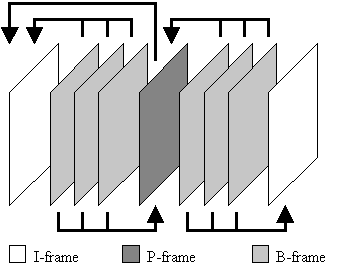
\includegraphics[width=0.5\textwidth]{graphics/ipb_frames.png}
%\end{figure}
}

\subsection{JPEG2000}
\frame{\frametitle{JPEG2000}
\begin{itemize}
 \item used as a baseline for comparison
 \item standard encoding settings, except number of layers
 \item ImageMagick with integrated OpenJPEG library
\end{itemize}
}

\subsection{Video Compression}
\frame{\frametitle{Video Compression}
\hspace{2cm}\huge Why video compression?
}

\frame{\frametitle{Video Compression}
	\underline{Why video compression?}
	\vspace{5mm}
	\begin{itemize}
		\item Very similar images
		\item Image compression only compresses individual images
		\item Video compression does 2 things:
		\begin{enumerate}
			\item Compresses images
			\item Exploits similarities between images
		\end{enumerate}
	\end{itemize}
}




\subsection{I,P,B-Frames}
\frame{\frametitle{I,P,B-Frames}
% http://www.tipterminal.de/pics/ipb_frames.gif
3 different types of pictures
\begin{itemize}
 \item I-Frame: Intra-coded picture
 \item P-Frame: Predictive-coded picture
 \item B-Frame: Bidirectional predictive-coded picture
\end{itemize}
\begin{figure}[H]
 \centering
 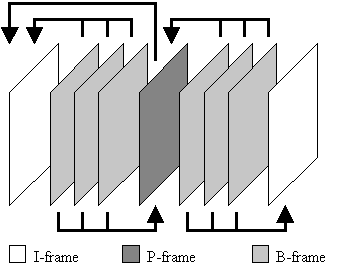
\includegraphics[width=0.5\textwidth]{graphics/ipb_frames.png}
\end{figure}
}

\subsection{Group Of Pictures}
\frame{\frametitle{Group Of Pictures}
\begin{itemize}
 \item usually defined with two numbers
 \begin{enumerate}
  \item defines distance of two I-Frames
  \item defines distance of two anchor frames (I or P)
 \end{enumerate}
 \item we used GOP to adapt the encoding to the database
 \begin{itemize}
  \item 24 pictures per person: use GOP 24 $\rightarrow$ 1 I-Frame per person
  \item 4 pictures per finger: use GOP 4 $\rightarrow$ 1 I-Frame per finger
 \end{itemize}
 \item P- and B-Frames allow higher compression $\rightarrow$ GOP affects the compression rate
\end{itemize}
}

\section{Section 2}
\subsection{Subsection 1}
\frame{\frametitle{Subsection 1}
Testtext 2.1
}

\section{CRF , Presets and Settings}
\frame{\frametitle{CRF}
\begin{itemize}
\item CRF value (Constant Rate Factor)
\begin{enumerate}
    \item The range of the quantizer scale is 0-51
    \item A lower value means better quality (0 for best quality, lossless)
    \item default value is 23
    \item A higher value means bad quality (51 for worst quality)
\end{enumerate}
\end{itemize}}

\frame{\frametitle{Presets}
\begin{itemize}
\item presets (they provide a certain encoding speed)
 \begin{enumerate}
   \item ultrafast , superfast , veryfast , faster , fast 
   \item medium (default)
   \item slow, slower, veryslow, placebo
   \item we focused more to the slower presets (medium-veryslow)
 \end{enumerate}
 \end{itemize}}
 
 \frame{\frametitle{Settings}
 \begin{itemize}
\item what are the settings behind them?
  

\begin{center}
\begin{tabular}{ |c|c|c| } 
 \hline
 slow & slower & veryslow \\
 \hline 
 \hline
 --b-adapt 2 & --b-adapt 2 & --b-adapt 2 \\
 \hline 
 --direct auto & --direct auto & --direct auto \\
 \hline
 default & default & --bframes 8\\
 \hline
 --me umh &  --me umh & --me umh \\
 \hline
 --rc-lookahead 50 & --rc-lookahead 60 & --rc-lookahead 60 \\
 \hline
 default & --partitions all & --partitions all \\
 \hline
 default & default & --merange 24 \\
 \hline
 --ref 5 & --ref 8 & --ref 16 \\
 \hline
 --subme 8 & --subme 9 & --subme 10\\
 \hline
 default & --trellis 2 & --trellis 2 \\
 \hline
\end{tabular}
\end{center}


      
\end{itemize}
 
}
 \frame{\frametitle{Settings}
  \begin{itemize}
    \item quick explanation of the settings :
    \begin{itemize}
        \item --rc-lookahead "Frames" : \\
        \begin{itemize}
        \item amount of macroblocktree and VBV algorithms
        \item higher value means that more memory and time is required
        
        \end{itemize}
        \item --b-adapt "Mod" : \\
        \begin{itemize}
        \item algorithm for the adaptive distribution of B-frames
        \item values : 0,1,2
        \end{itemize}
        \item --direct "Mod" : \\
        \begin{itemize}
        \item  temporal or spatial information is used in B frames
        \end{itemize}
        \item --bframes "Max" : \\
        \begin{itemize}
        \item Defines how many B-frames can be positioned directly behind each other
        \item values are between 0 and 16 (3 is default)
        \end{itemize}
        \item --me "mod" : \\
        \begin{itemize}
        \item Algorithm for motion search
        \end{itemize}
        
        
    \end{itemize}
  \end{itemize}
 }
\frame{\frametitle{Settings}
\begin{itemize}
\item --partitions "partitions" :\\
        \begin{itemize}
        \item partition size for macroblocks
        \end{itemize}
\item --merange "radius" : \\
        \begin{itemize}
        \item size of the area
        \end{itemize}
    \item --ref "frames" : \\
    \begin{itemize}
    \item amount of valid reference frames
    \end{itemize}
    \item --subme "quality" : \\
    \begin{itemize}
    \item Defines the quality level for the subpixel motion search and the partition decision
    \end{itemize}
    
\end{itemize} 
}

\section{Implementation}

\subsection{JPEG2000 Compression}
\frame{\frametitle{JPEG2000 Compression}


}

\subsection{Video Compression}
\frame{\frametitle{Video Compression}
	Setup:
	\begin{itemize}
		\item Used ffmpeg v.3.3.2 (latest version)
		\item Compressed 240 images
		\item Different crf values (0-50)
		\item Varying group of pictures (1, 4, 24)
		\item two presets (medium, veryslow)
	\end{itemize}
	
	
}

\frame{\frametitle{Video Compression}
	Repeat for each (crf, gop, preset) - combination
	\begin{enumerate}
		\item Compress images into single video
		\item get videosize (for compression rate)
		\item Decompress video $\rightarrow$ get images
		\item Put into folder named with settings
	\end{enumerate}
	Additional steps
	\begin{itemize}
		\item Collect image names $\rightarrow$ parameters for matcher
		\item rename decompressed videos
	\end{itemize}
	
	
}

\subsection{Matching}
\frame{\frametitle{Matching}
	
	
}


\section{Results}

\end{document}





















